	Diamond turning is the name given to a turning process using diamond as the cutting tool. The tip of the tool bit can be either made of natural or synthetic diamond \cite{gerchman1986}.
	
	Although the process is sometimes called \textbf{single-point diamond turning (SPDT)}, it also refers to tools with radiused noses or other forms \cite{gerchman1986}. It is used to manufacture high-quality mold inserts, which are then used for molding plastic optical elements. Sometimes prototypes can be turned directly on plastic, to save the time and resources used on the mold insert turning. It can also be used for turning crystals. These optical parts are used in telescopes, video projectors, missile guidance systems, lasers, scientific research instruments, among other applications.\newline
	
	\begin{figure}[H]
		\centering
		\captionsetup{justification=centering}
		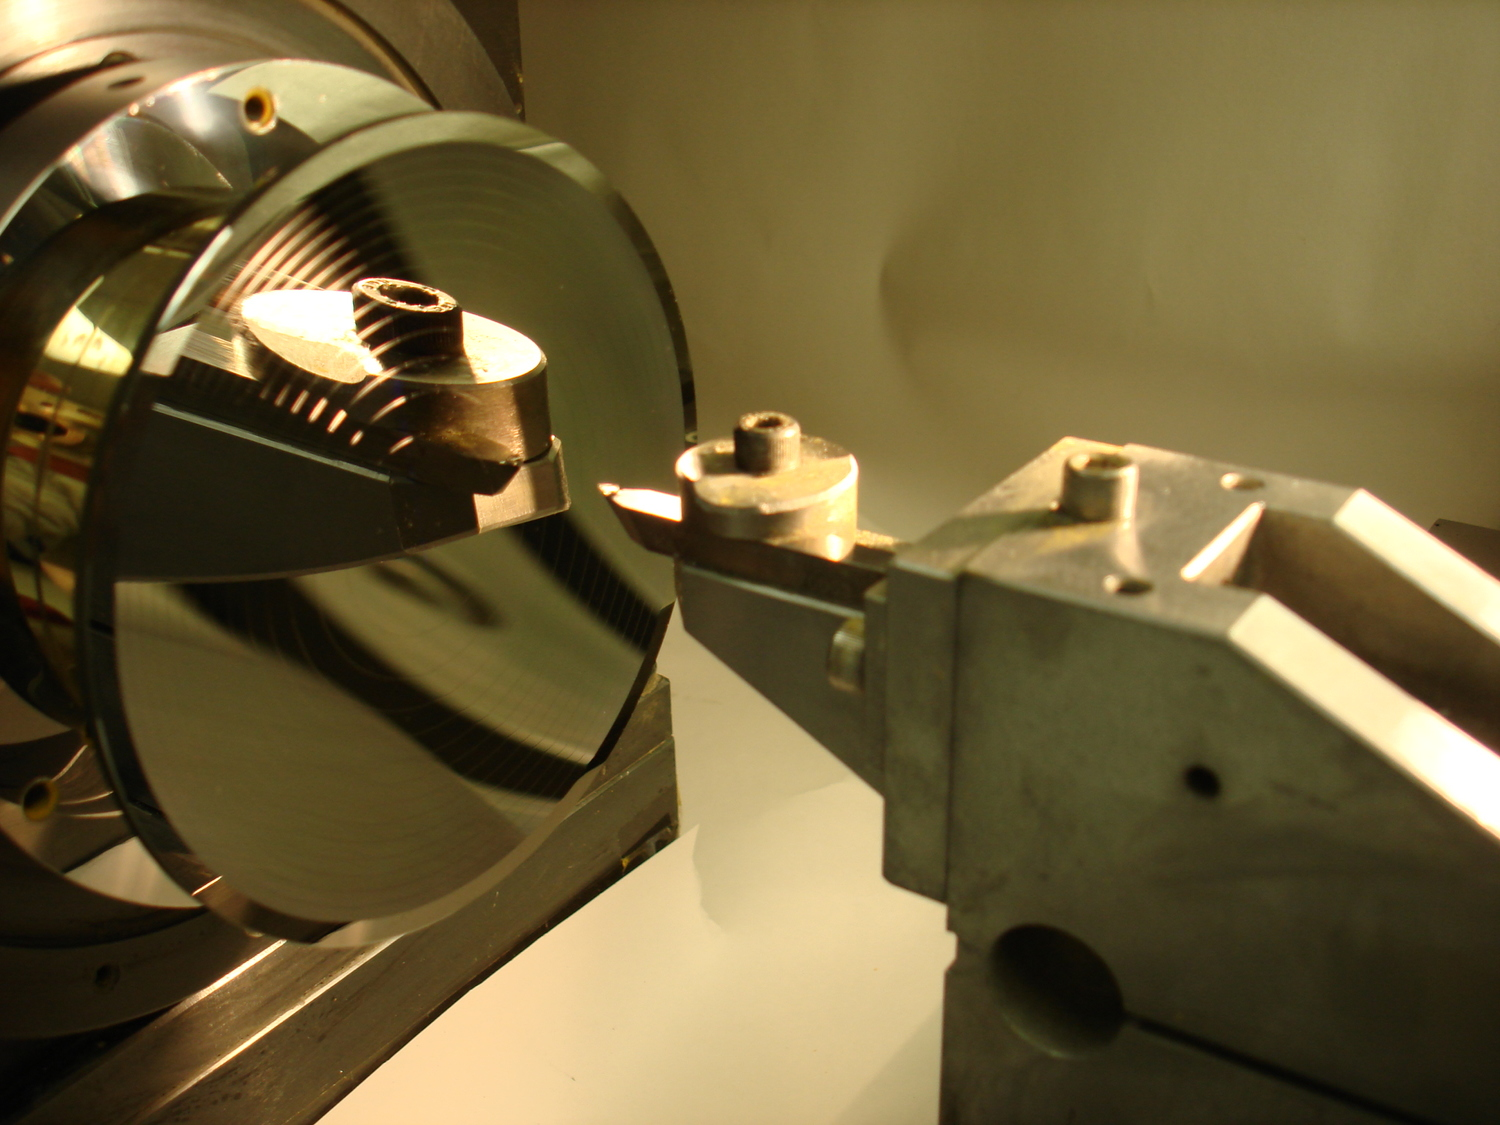
\includegraphics[width=0.8\linewidth]{Cap2/Diamondturning/piecewithtool.jpg}
		\caption{Diamond turning of a concave mirror.}
		\label{fig:piecewithtool}
	\end{figure}
	
	The machining with mono crystalline diamond tools is a cutting process which allows for ultra-precision quality surfaces with low nanometer scale roughness, because of its sharp cutting edge \cite{taniguchi1983}. Because of the single crystal structure,  diamond tools can be sharpened to have cutting edge rounding down to 20 nanometers, while conventional cutting tools can only go down to the micrometer scale. This enables optical surface with low nanometer roughness to be generated relatively independent of the machining parameters \cite{cheung2001}.
	
	\begin{figure}[H]
		\centering
		\captionsetup{justification=centering}
		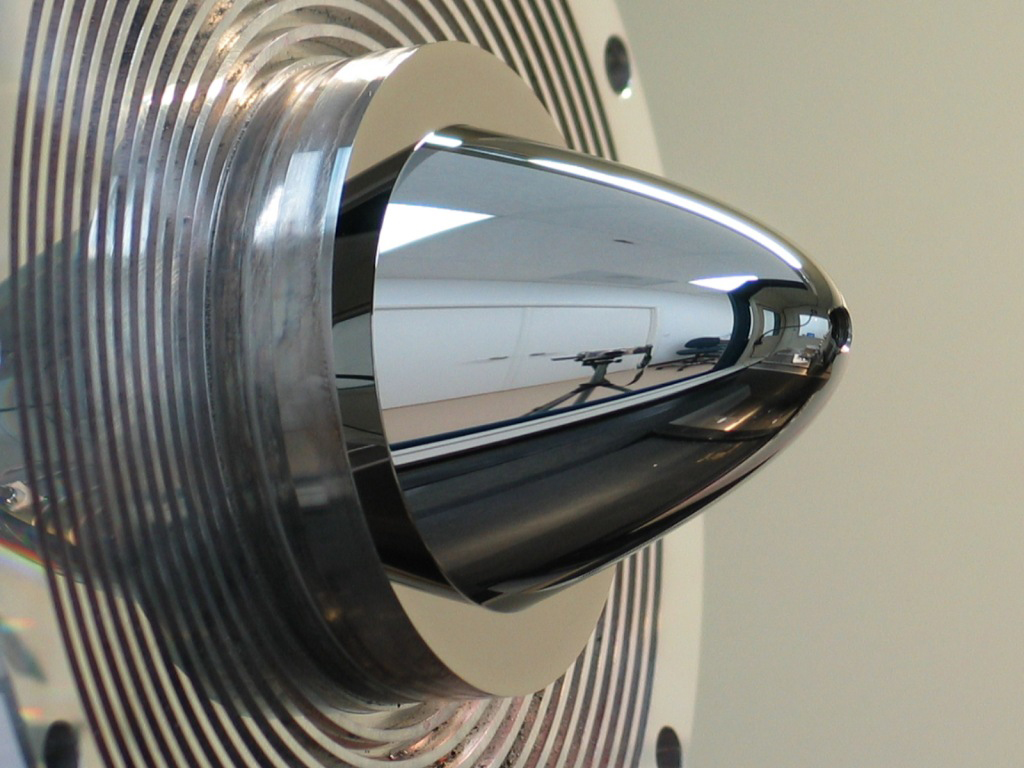
\includegraphics[width=0.8\linewidth]{Cap2/Diamondturning/mandrel.jpg}
		\caption{Metal mandrel turned with a diamond tool.}
		\label{fig:mandrel}
	\end{figure}
	
	It offers great surface quality with a vast range of materials, like non-ferrous metals, plastics and crystalline materials such as silicon and magnesium fluoride \cite{gerchman1986}. Diamond, being on of the hardest materials available, allows for a long standing time and its sharpness allows for low cutting forces during the process, which is key to avoid excessive vibration and to obtain a good surface finish. The mono crystal property is also essential, as it provides a tool without structural defects.
	
	This method offers a large geometrical freedom in the machining of continuous surfaces. Spheres, aspheres, freeform surfaces and microstructures can be easily machined with great results, as can be seen in Figures~\ref{fig:piecewithtool} and \ref{fig:mandrel}. Discontinuous surfaces, such as Fresnel structures and diffractive optical elements, can also be machined. With appropriate machines and corrections, a dimensional accuracy of less than 250 nm can be reached, as well as a surface roughness Ra of down to 1 nm \cite{cheung2001}.
	
	However, the main limitation of this technique is that it cannot be used for the machining of ferrous metals. The carbon in the diamond tool has a big chemical affinity with these metals, and a high degree of carbon diffusion occurs from the tool to the workpiece when these two materials make contact. This causes a high amount of tool wear, enormously decreasing the life of the tool, which is very expensive, thus making the process unfeasible \cite{paul1996,thornton1978}.
	
	Two main lines of research have been conducted on recent years to overcome this limitation. One of them consists on imposing a bidirectional vibration on the tool, causing the tool tip to describe an elliptical Lissajous figure. The idea is to make the contact time between tool and part decrease and reduce the wear process of the diamond tool. The vibration must occur on a very high frequency, often in the ultrasonic range, so that it moves fast and does not maintain contact with the surface for too long. The process is illustrated on Figure~\ref{fig:toolvibration}. To accomplish the correct vibration pattern, the right geometry of the tool holder must be used to obtain an adequate resonance. One of the leading companies on this topic is Innolite, based in Aachen, Germany.\newline
	
	\begin{figure}[H]
		\centering
		\captionsetup{justification=centering}
		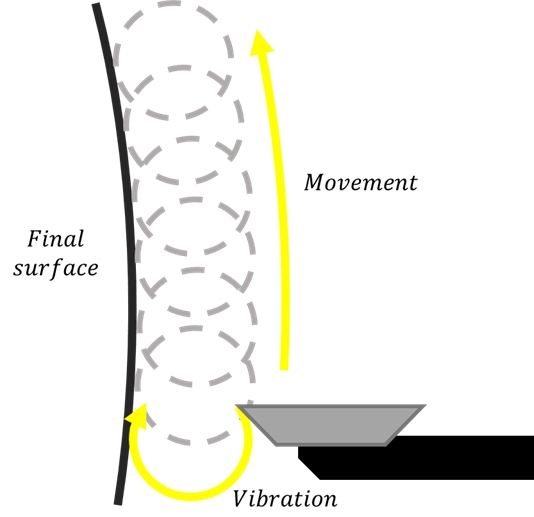
\includegraphics[width=0.7\linewidth]{Cap2/Diamondturning/toolvibration.jpg}
		\caption{Tool vibration pattern for machining of ferrous metals with diamond-tipped tools.}
		\label{fig:toolvibration}
	\end{figure}
	
	%The second line of research consists on applying a voltage between the tool and the piece, thus causing a current to run through the interface, to make ferrous metals diamond-workable \cite{}. It has shown some promising results, but still not enough for commercial applications to be developed and used in larger scale.
	\newpage